%%%%%%%%%%%%%%%%%%%%%%%%%%%%%%%%%%%%%%%%%
% Short Sectioned Assignment LaTeX Template Version 1.0 (5/5/12)
% This template has been downloaded from: http://www.LaTeXTemplates.com
% Original author:  Frits Wenneker (http://www.howtotex.com)
% License: CC BY-NC-SA 3.0 (http://creativecommons.org/licenses/by-nc-sa/3.0/)
%%%%%%%%%%%%%%%%%%%%%%%%%%%%%%%%%%%%%%%%%

%----------------------------------------------------------------------------------------
%   PACKAGES AND OTHER DOCUMENT CONFIGURATIONS
%----------------------------------------------------------------------------------------

\documentclass[10pt,a4paper,spanish]{article}

% ---- Entrada y salida de texto -----

\usepackage[spanish]{babel} 
\usepackage[T1]{fontenc} % Use 8-bit encoding that has 256 glyphs
\usepackage[utf8]{inputenc}
\usepackage{minted}
% \usepackage{fourier} % Use the Adobe Utopia font for the document - comment this line to return to the LaTeX default
\usepackage[usenames, dvipsnames]{color}
\usepackage{xcolor}
\usepackage{colortbl}
\usepackage[bookmarks=true,colorlinks=true,linkcolor=red,citecolor=blue]{hyperref}
\usepackage{cite}
\usepackage[official]{eurosym}
\usepackage{tikz}
\usepackage{pgfplots}
\pgfplotsset{compat=1.5}
\usepackage{pgf-pie}
\usepackage{subfigure}

% ---- Otros paquetes ----
\usepackage{enumerate}
\usepackage{amsmath,amsfonts,amsthm,amssymb} % Math packages
\usepackage{graphics,graphicx} %para incluir imágenes y notas en las imágenes
% Para hacer tablas comlejas
%\usepackage{multirow}
%\usepackage{threeparttable}

\usepackage[a4paper, margin=1.3in]{geometry}


\usepackage{sectsty} % Allows customizing section commands
\allsectionsfont{\centering \normalfont\bfseries\scshape} % Make all sections centered, the default font and small caps

\usepackage{fancyhdr} % Custom headers and footers
\pagestyle{fancyplain} % Makes all pages in the document conform to the custom headers and footers
\fancyhead{} % No page header - if you want one, create it in the same way as the footers below
\fancyfoot[L]{} % Empty left footer
\fancyfoot[C]{} % Empty center footer
\fancyfoot[R]{\thepage} % Page numbering for right footer
\renewcommand{\headrulewidth}{0pt} % Remove header underlines
\renewcommand{\footrulewidth}{0pt} % Remove footer underlines
\setlength{\headheight}{13.6pt} % Customize the height of the header

\numberwithin{equation}{section} % Number equations within sections (i.e. 1.1, 1.2, 2.1, 2.2 instead of 1, 2, 3, 4)
\numberwithin{figure}{section} % Number figures within sections (i.e. 1.1, 1.2, 2.1, 2.2 instead of 1, 2, 3, 4)
\numberwithin{table}{section} % Number tables within sections (i.e. 1.1, 1.2, 2.1, 2.2 instead of 1, 2, 3, 4)

\setlength\parindent{0pt} % Removes all indentation from paragraphs - comment this line for an assignment with lots of text
\setlength{\parskip}{1ex plus 0.5ex minus 0.2ex}

\newcommand{\horrule}[1]{\rule{\linewidth}{#1}} % Create horizontal rule command with 1 argument of height

%----------------------------------------------------------------------------------------
%   TÍTULO Y DATOS DEL ALUMNO
%----------------------------------------------------------------------------------------

\title{
\normalfont \normalsize 
\textsc{{\bf Ingeniería de Servidores (2015-2016)} \\ Grado en Ingeniería Informática \\ Universidad de Granada} \\ [25pt] % Your university, school and/or department name(s)
\horrule{0.5pt} \\[0.4cm] % Thin top horizontal rule
\huge Memoria Práctica 1 \\ % The assignment title
\horrule{2pt} \\[0.5cm] % Thick bottom horizontal rule
}

\author{Marta Gómez Macías} % Nombre y apellidos

\date{\normalsize\today} % Incluye la fecha actual


%----------------------------------------------------------------------------------------
% DOCUMENTO
%----------------------------------------------------------------------------------------

\begin{document}
%Cambiar Cuadros por Tablas y lista de...
\renewcommand{\listtablename}{Índice de tablas}
\renewcommand{\tablename}{Tabla} 

\maketitle % Muestra el Título
\pagenumbering{gobble} 

\newpage %inserta un salto de página
\pagenumbering{arabic} 

\tableofcontents % para generar el índice de contenidos

\listoffigures

\listoftables

\newpage

%----------------------------------------------------------------------------------------
%   Cuesti´on 1
%----------------------------------------------------------------------------------------

\section{¿Qué modos y/o tipos de ``virtualización'' existen?}
Hoy en día hay tres tipos de virtualización, tal y como se cita en \cite{vmware}:
\begin{enumerate}[$\bigstar$]
    \item Virtualización completa usando traducción binaria
    \item Virtualización asistida por el sistema operativo o \textit{paravirtualización}
    \item Virtualización asistida por el hardware
\end{enumerate}

\subsection{Virtualización completa usando traducción binaria}
Este tipo de virtualización, para obtener un mayor rendimiento, ejecuta el código de usuario directamente sobre el hardware. En cambio, el código con instrucciones privilegiadas debe ser traducido primero por el monitor de máquina virtual a instrucciones hardware, esto se ve muy bien en la \hyperref[full_vir]{Figura \ref*{full_vir}}.

Es el único tipo de virtualización que abstrae completamente el sistema operativo y que no necesita asistencia hardware ni software. Por eso, el sistema operativo no necesita ser modificado.

\begin{figure}[!h]
\centering
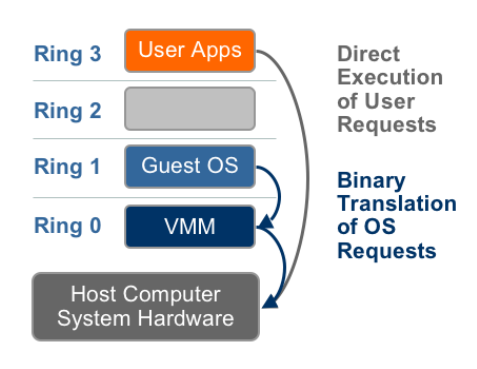
\includegraphics[width=0.5\textwidth]{1}
\caption{Esquema de la virtualización completa usando traducción binaria}
\label{full_vir}
\end{figure}

\subsection{Virtualización asistida por el sistema operativo o \textit{Paravirtualización}}
La paravirtualización implica modificar el sistema operativo virtualizado para reemplazar las instrucciones privilegiadas por llamadas a la capa de virtualización. Por esto, tiene poca compatibilidad y portabilidad. Al igual que en el anterior tipo, las aplicaciones de usuario se ejecutan directamente en el hardware. El esquema de este tipo de virtualización se ve en la \hyperref[paravir]{Figura \ref*{paravir}}.

\begin{figure}[!h]
\centering
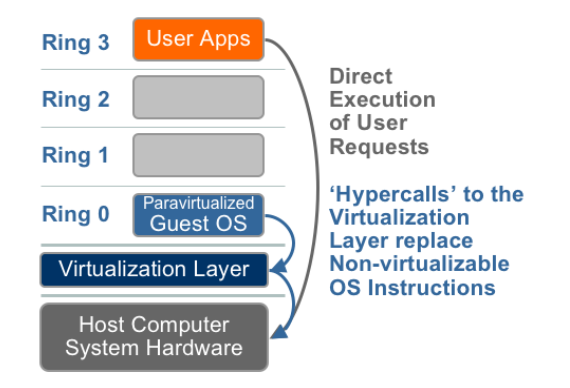
\includegraphics[width=0.5\textwidth]{2}
\caption{Esquema de la paravirtualización}
\label{paravir}
\end{figure}

Tal y como se explica en \cite{amazon}, la paravirtualización solía dar mejores resultados que la virtualización completa en operaciones de acceso a memoria y red porque tenían drivers de entrada salida especializados que evitaban la sobrecarga de emular éstas operaciones, cosa que no pasa en la virtualización completa donde tenemos que traducir las instrucciones. Desde que estos drivers están disponibles también para virtualización completa, la virtualización completa ofrece los mismos o mejores resultados que la paravirtualización.

\subsection{Virtualización asistida por el hardware}
Los desarrolladores hardware han desarrollado procesadores que permiten al monitor de máquina virtual ejecutarse en un modo root por debajo del sistema operativo y por encima del hardware. Así, como se ve en la \hyperref[virast]{Figura \ref*{virast}}, el monitor capta las instrucciones privilegiadas y no hay por qué aplicarles una traducción binaria o paravirtualizarlas.

\begin{figure}[!h]
\centering
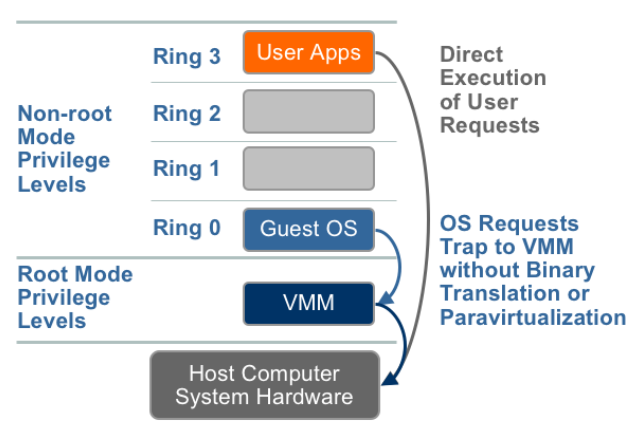
\includegraphics[width=0.5\textwidth]{3}
\caption{Esquema de la virtualización asistida por el hardware}
\label{virast}
\end{figure}

\section{Muestre los precios y características de varios proveedores de VPS (\textit{Virtual Private Server}) y compare con el precio de servidores dedicados (administrados y no administrados). Comente diferencias.}
Se ha comparado los precios de dos proveedores: \href{https://www.hosteurope.es/}{Host Europe} y \href{http://www.hostalia.com/}{Hostalia}

\subsection{Host Europe (\textit{Red Coruña})}
\subsubsection{VPS}
Host Europe nos ofrece tres tipos de servidores VPS según nuestras necesidades, o bien con disco duro SSD o con SATA, como se indica en \cite{hevps}.

Todos los servicios incluyen \textbf{tráfico ilimitado}.

Si escogemos un disco duro SATA para nuestro servidor los precios serían:

\begin{table}[!h]
\begin{tabular}{l | c | c | c }
 & Alpha $\alpha$ & Delta $\delta$ & Omega $\omega$ \\
 \hline
 RAM garantizada & 2 GB & 4 GB & 8 GB \\
 RAM dinámica & 4 GB & 8 GB & 16 GB \\
 Espacio en disco & 200 GB SATA & 400 GB SATA & 600 GB SATA \\
 Precio & 9,74\euro/mes & 19,49\euro/mes &  25,99\euro/mes \\
 \end{tabular}
 \caption{Precios en Host Europe por un servidor VPS con disco duro SATA}
 \label{hevpssata}
 \end{table}

En cambio, si escogemos un disco duro SSD, varían los siguientes parámetros:

\begin{table}[!h]
\begin{tabular}{l | c | c | c }
 & Alpha $\alpha$ & Delta $\delta$ & Omega $\omega$ \\
 \hline
 Espacio en disco & 100 GB SSD & 200 GB SSD & 300 GB SSD \\
 Precio & 11,04\euro/mes & 21,44\euro/mes &  29,24\euro/mes \\
 \end{tabular}
 \caption{Precios en Host Europe por un servidor VPS con disco duro SSD}
 \label{hevpsssd}
 \end{table}

 \subsubsection{Servidores dedicados}
 En cuanto a servidores dedicados, tal y como se explica en \cite{hese}, hay cuatro tipos de servidores dedicados, en todos podemos elegir entre servidores con Linux o con Windows. Además, los servidores con Linux son 100\% administrados por el equipo de Host Europe gratuitamente.

 Si los elegimos con Linux (\textit{CentOS 6}), los precios serían (con procesador \textit{Intel Xeon E3-1230} menos $\delta$ con \textit{Intel Xeon E3-1270}):
\begin{table}[!h]
\begin{tabular}{l | c | c | c | c}
 & Alpha $\alpha$ & Gamma $\gamma$ & Delta $\delta$ & Omega $\omega$ \\
\hline
RAM & 8 GB DDR3 & 16 GB DDR3 & 32 GB DDR3 & 64 GB DDR3 \\
Discos duros & 2 $\times$ 1 TB & 2 $\times$ 2 TB & 2 $\times$ 600 GB & 4 $\times$ 600 GB \\
Precio & 64,99\euro/mes & 77,99\euro/mes & 103,99\euro/mes & 149,49 \euro/mes \\
\end{tabular}
\caption{Precios en Host Europe por un servidor dedicado con Linux}
\label{heselin}
\end{table}

Si escogemos Windows, tenemos las mismas prestaciones (RAM, procesador y disco duro) pero nos dan a elegir entre varias distribuciones Windows:

\begin{table}[!h]
\begin{tabular}{l | c | c | c | c}
 & Alpha $\alpha$ & Gamma $\gamma$ & Delta $\delta$ & Omega $\omega$ \\
\hline
2008 Std. ed. & 77,99\euro/mes & 90,99\euro/mes & 116,99\euro/mes & 162,49\euro/mes \\
2008 Web ed. & 71,49\euro/mes & 84,49\euro/mes & 110,49\euro/mes & 155,99\euro/mes \\
2012 Std. ed. & 77,99\euro/mes & 90,99\euro/mes & 116,99\euro/mes & 162,49\euro/mes \\
\end{tabular}
\caption{Precios en Host Europe por un servidor dedicado con las distintas versiones de Windows}
\label{hesewin}
\end{table}

En la relación prestaciones/precio, el servidor VPS da mejor resultado. Ya que con unas prestaciones (aunque un poco inferiores) parecidas, cuesta más de la mitad que un servidor dedicado. 

\subsection{Hostalia}
\subsubsection{VPS}
Tal y como se explica en \cite{hvps}, podemos elegir entre tres tipos de servidores virtuales VPS.

Todos incluyen una transferencia de \textbf{1.000 GB}.

\begin{table}[!h]
\begin{tabular}{l | c | c | c }
 & VPS Base & VPS Avanzado &  VPS Plus \\
 \hline
 Espacio en disco & 25 GB & 50 GB & 100 GB \\
 Memoria RAM & 1 GB & 2 GB & 3 GB \\
 Precio & 11,21\euro/mes & 18,71\euro/mes & 26,21\euro/mes \\
\end{tabular}
\caption{Precios en Hostalia por un servidor VPS.}
\label{hostvps}
\end{table}

\subsubsection{Servidores dedicados}
En este caso, tal y como se especifica en \cite{hse}, podemos elegir entre cuatro tipos de servidores, cada uno con unas características muy diferentes.

\begin{table}[!h]
\begin{tabular}{l | c | c | c | c}
 & Start & Advanced & Professional & Premium \\
 \hline
 Procesador & 1 $\times$ E3-1241 & 1 $\times$ E5-2420 & 1 $\times$ E5-2640 & 2 $\times$ E5-2640 \\
 Cores / núcleos $\times$ velocidad & 4 $\times$ 3,5 GHz & 6 $\times$ 2,2Ghz & 8 $\times$ 2,6 GHz & 16 $\times$ 2,6Ghz \\
 Memoria RAM & 16 GB & 32 GB & 64 GB & 128 GB \\
 Disco Duro & 2 $\times$ 1TB SATA & 2 $\times$ 1TB SATA & 2 $\times$ 1TB SATA & 2 $\times$ 1TB SATA\\
 Disco SSD & - & 200, 400 y 800 GB & 200, 400 y 800 GB & 200, 400 y 800 GB \\
 Precio & 69,90\euro/mes & 99,90\euro/mes & 199,90\euro/mes & 269,90\euro/mes \\
\end{tabular}
\caption{Precios en Hostalia por un servidor dedicado.}
\label{hostse}
\end{table}

En Hostalia, la diferencia de prestaciones entre un servidor VPS y uno dedicado es enorme, también lo es la diferencia de precio. Pues pasamos de pagar unos 20\euro/mes a pagar más de 100.

\subsection{Conclusiones}
Para comparar los servidores VPS de ambas compañías, se ha hecho uso de las tablas \hyperref[hevpssata]{\ref*{hevpssata}} y \hyperref[hostvps]{\ref*{hostvps}}.

En cuanto a prestaciones en VPS se refiere, Host Europe merece mucho más la pena tanto en prestaciones como en precio. Por ejemplo, el servidor VPS más básico de Host Europe nos da 2GB de RAM y 200GB de espacio en disco por unos 10\euro/mes, mientras que el más básico de Hostalia, nos da 1GB de RAM y 25GB de almacenamiento en disco por unos 11\euro/mes. Para conseguir las prestaciones que nos da el servidor VPS más barato de Host Europe, en Hostalia tenemos que irnos al servidor VPS más caro y pagar unos 26\euro/mes.

Para comparar los servidores dedicados de ambas compañías, se ha hecho uso de las tablas \hyperref[heselin]{\ref*{heselin}} y \hyperref[hostse]{\ref*{hostse}}.

En cuanto a prestaciones en servidores dedicados, están las dos al mismo nivel. Por ejemplo, comparando los servidores básicos de cada compañía vemos que en Host Europe tenemos 8GB de RAM, 2 TB de disco duro y un procesador por 65\euro/mes, mientras que en Hostalia, un procesador, 16 GB de RAM y 2 TB de disco duro por 70\euro/mes. Es decir, pagando un poco más, tenemos el doble de memoria RAM. 

Comparando los servidores ``Professional'' de Hostalia y ``Omega $\omega$'' de Host Europe, vemos que tienen prestaciones muy parecidas, pero en Hostalia pagamos 50\euro/mes más. De hecho, en Host Europe nos ofrecen 2,4 TB de espacio en disco mientras que en Hostalia sólo 2 TB. Así que, en este caso, pagando menos conseguimos más.

\newpage
\section{¿Qué otros software de virtualización existen además de VMWare y Virtual Box?}
Existen numerosos software de virtualización. A continuación se muestran dos ejemplos:
\subsection{Windows Virtual PC}
Es un software de virtualización que se basa en la \textbf{Paravirtualización}. Tal y como se indica en \cite{windowsvpc}, soporta como sistema operativo Host las distintas versiones de \textbf{Windows 7} (Home Basic, Professional, Enterprise, etc.) y permite virtualizar los siguientes sistemas operativos:
\begin{enumerate}[$\bullet$]
    \item Windows XP Service Pack 3 (SP3) Professional
    \item Windows Vista Enterprise Service Pack 1 (SP1)
    \item Windows Vista Ultimate Service Pack 1 (SP1)
    \item Windows Vista Business Service Pack 1 (SP1)
    \item Windows 7 Professional
    \item Windows 7 Ultimate
    \item Windows 7 Enterprise
\end{enumerate}

\subsection{OpenVZ}
Tal y como se explica en \cite{openvz}, OpenVZ es un software que permite crear VPSs con sistemas operativos Linux sobre un servidor. Cada contenedor es totalmente independiente de los demás y no es consciente de que está siendo virtualizado. Tiene licencia GNU GPL.

\section{Enumere algunas de las innovaciones en Windows 2012R2 respecto a 2008R2}
En \cite{comws2012}, se compara Windows Server 2012R2 con las versiones anteriores de Windows Server. En comparación a la versión 2008R2, tenemos como resultado que la versión 2012R2 tiene una capacidad de procesamiento y de almacenamiento mayor a la versión 2008R2 tal y como se refleja en la \hyperref[prest]{Tabla \ref*{prest}}.

\begin{table}[!h]
\begin{tabular}{c | c | c | c}
Sistema & & Windows Server 2008R2 & Windows Server 2012R2 \\
\hline
\textbf{Host} & Procesadores Lógicos & 64 & 320 \\
& Memoria física & 1 TB & 4 TB \\
& Procesadores virtuales por host & 512 & 2048 \\
\hline
\textbf{Máquina virtual} & Procesadores virtuales por VM & 64 GB & 1 TB \\
& Capacidad de disco virtual & 2 TB & 64 TB \\
& Máquinas virtuales activas & 384 & 1024 \\
\hline
\textbf{Clúster} & Nodos & 16 & 64 \\
& Máquinas virtuales & 1000 & 8000 \\
\end{tabular}
\caption{Comparación entre las prestaciones de Windows Server 2008R2 y Windows Server 2012R2}
\label{prest}
\end{table}

Pero no sólo se compara el rendimiento en \cite{comws2012}, también se compara funcionalidad. Algunas de las funcionalidades que incluye la versión 2012R2 como novedad son:
\begin{enumerate}[$\bullet$]
    \item \textbf{Administración de direcciones IP}
    \item \textbf{Control de acceso dinámico}: Tal y como se dice en \cite{cad}, el control de acceso dinámico nos permite restringir el acceso a los archivos de nuestra empresa y controlar quien ha accedido a ellos. Para ello, podemos etiquetar los distintos datos que tenemos, controlar el acceso a los archivos, encriptar documentos \textit{office} confidenciales, etc.
    \item \textbf{Escalabilidad compatible con NUMA}\footnote{NUMA: Not-Uniform Memory Access, es decir, multiprocesadores con acceso a memoria no uniforme. Los más escalables debido a que cada uno tiene ``su'' módulo de memoria, aunque puede acceder a los módulos de memoria de otros procesadores.}
    \item \textbf{Administración multiservidor}
\end{enumerate}

\section{¿Qué empresa hay detrás de Ubuntu? ¿Qué otros productos/servicios ofrece?}
Si entramos en la sección ``Partners'' en la \href{http://partners.ubuntu.com/}{página web de Ubuntu} y hacemos scroll, veremos una sección en la que se dice que detrás de Ubuntu, está \textbf{Canonical}.

Tal y como indica en \cite{sercan}, Canonical ofrece un servicio para empresas llamado \textbf{\textit{Ubuntu Advantage}}. En la página web de Ubuntu, \cite{ua}, lo describen como un paquete profesional de soporte por parte de ingenieros de Canonical para ayudar a empreas a gestionar sus sistemas con Ubuntu. Incluye cosas como servicio telefónico todos los días a todas horas, acceso a \textit{Landscape}\footnote{Una herramienta de gestión para automatizar actualizaciones y gestionar sistemas físicos, virtuales y cloud.}, etc.

\section{¿Qué relación tiene CentOS con Red Hat y el proyecto Fedora?}
En Enero de 2014, se anunció en la página de CentOs, \cite{centos}, que Red Hat se iba a unir al desarrollo de esta distribución. Respecto al proyecto Fedora, en la sección \textit{Our Community} de \cite{fedora}, se dice que en el desarrollo de dicho proyecto participan los empleados de Red Hat, por tanto, al estar Red Hat relacionado en el desarrollo de ambas distribuciones se entiende que ambas están relacionadas.

\section{Indique qué otros SO se utilizan en servidores y el porcentaje de uso.}
Según se indica en \cite{osser}, el porcentaje de uso es el indicado en la \hyperref[osser]{Figura \ref*{osser}}.

\begin{figure}[!h]
\centering
\begin{tikzpicture}[scale=0.6]
\pie[text=legend]{67.3/Unix, 32.8/WIndows}
\end{tikzpicture}
\caption{Porcentaje de uso de Unix y Windows en servidores}
\label{osser}
\end{figure}

De ese 67,3\%, en \cite{unixser} se indica que el porcentaje de uso de cada sistema operativo basado en Unix es el de la \hyperref[unixser]{Figura \ref*{unixser}}.

\begin{figure}[!h]
\centering
\begin{tikzpicture}[scale=0.6]
\pie[text=legend]{53/Linux, 13/BSD, 45.6/Desconocido, 0.3/Otros}
\end{tikzpicture}
\caption{Porcentaje de uso de sistemas operativos basados en Unix en servidores}
\label{unixser}
\end{figure}

Por último, de ese 53\% que usa Linux en su servidor, tal y como muestra \cite{linuxser} el porcentaje de uso de cada distribución es el mostrado en la \hyperref[linuxser]{Figura \ref*{linuxser}}.

\begin{figure}[!h]
\centering
\begin{tikzpicture}[scale=0.7]
\pie[text=legend]{31.7/Debian, 30/Ubuntu, 20.7/CentOS, 4.3/Red Hat, 2.1/Gentoo, 1.3/Fedora, 1.1/SuSe, 0.8/Otros, 8.6/Desconocido}
\end{tikzpicture}
\caption{Porcentaje de uso de Linux en servidores}
\label{linuxser}
\end{figure}

\section{¿Qué diferencia hay entre RAID mediante software y mediante hardware?}
En \cite{intelraid} se comparan las diferencias entre los RAID software y los RAID hardware.

Aunque los RAID software son más baratos, sólo pueden responder ante errores en el disco duro, pero no cuando falla el sistema operativo o el servidor. En cambio, los RAID hardware sí, porque incluyen una cache y una batería. Los RAID software no pueden porque guardan sus datos en la cache del sistema operativo.

Para ver porqué se ha producido un error, debemos reiniciar el sistema, al guardar los RAID hardware los informes de errores en su cache, si el sistema falla o se cae no los perderemos, mientras que con los RAID software sí.

En cuanto a rendimiento, aunque antes los RAID software afectaban notablemente al rendimiento del sistema, con las potentes CPUs que tenemos hoy en día el rendimiento obtenido por los RAID software puede compararse con el obtenido por los RAID hardware. Sin embargo, en operaciones de E/S los RAID hardware son hasta 100 veces más rápidos que los RAID software.

Finalmente, en cuanto a la virtualización de servidores, los RAID hardware son mucho mejores que los software. Ésto es a que para poder usar RAID software deberíamos tener una instancia de la pila del RAID software en cada servidor virtualizado.

\section{a) ¿Qué es LVM? b) ¿Qué ventaja tiene para un servidor de gama baja? c) Si va a tener un servidor web, ¿le daría un tamaño grande o pequeño a /var?}
\begin{enumerate}[a)]
    \item Tal y como se explica en \cite{lvmubuntu}, LVM son las siglas de \textit{Logical Volume Management}. LVM es un sistema de gestión de volúmenes lógicos (o sistemas de archivos), lo cual es mucho mejor que el método tradicional consistente en dividir el disco duro en segmentos y formatear la partición deseada con un sistema de archivos.
    \item Una gran ventaja es que podemos realizar cambios mientras el sistema está en funcionamiento.
    \item En \cite{linuxvar}, se explica que el directorio /var contiene datos del software que se está ejecutando en el sistema. Ya que un servidor web guarda logs, archivos de bases de datos y documentos web, /var debería tener un tamaño grande.
\end{enumerate}

\section{¿Debemos cifrar también el volumen que contiene el espacio para swap? ¿y el volumen en el que montaremos /boot?}
Sí, como se indica en \cite{enswap}, si no ciframos el espacio para \textit{swap}, tendremos información que hemos cifrado en los otros discos, pero sin cifrar. Por tanto, nuestro esfuerzo por proteger nuestra información será en vano. En cambio, no deberemos cifrar el volumen en el que montaremos \textit{/boot}, ya que, tal y como se explica en \cite{enboot}, si criframos nuestra partición boot tendremos que tener un dispositivo aparte para desencriptarla (por ejemplo, un USB).

\section{¿Qué otro tipo de usos de una partición le permite configurar el asistente de instalación? ¿Cuál es la principal diferencia entre ext4 y ext2?}
Tal y como se ve en la \hyperref[usos_p]{Figura \ref*{usos_p}}, podemos usar una partición o bien como un \textbf{sistema de archivos} (ext4, ext2, btrfs, JFS, XFS, FAT16 o FAT32), o bien como \textbf{área de intercambio}, o bien como \textbf{volumen físico para la LVM}.

\begin{figure}[!h]
\centering
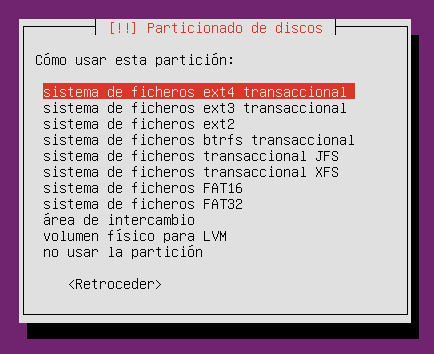
\includegraphics[width=0.4\textwidth]{4}
\caption{Usos posibles de una partición}
\label{usos_p}
\end{figure}

En cuanto a las principales diferencias entre ext4 y ext2, según \cite{ext4}, nos permite usar sistemas de archivos mayores a 16TB; se reducen los accesos a memoria y por tanto, las lecturas son más eficientes; además, el sistema de arhivos es más robusto frente a fallos en el disco y permite guardar archivos más grandes, entre otras cosas más.

\section{Muestre cómo ha quedado el disco particionado una vez el sistema está instalado (\textit{lsblk})}

Tras ejecutar el comando \textit{lsblk}, obtenemos el resultado que se muestra en la \hyperref[lsblk]{Figura \ref*{lsblk}}

\begin{figure}[!h]
\centering
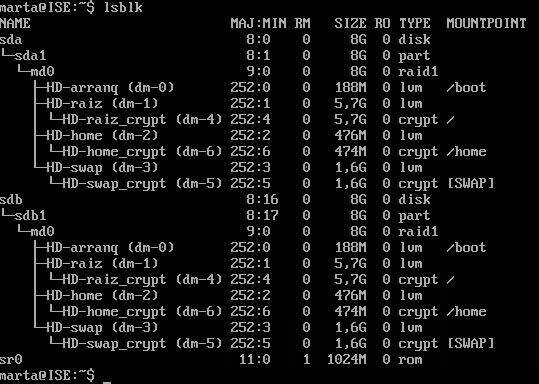
\includegraphics[width=0.7\textwidth]{6}
\caption{Resultado tras ejecutar el comando lsblk en la instalación de Ubuntu Server}
\label{lsblk}
\end{figure}

\section{a) ¿Cómo ha hecho el disco 2 ``arrancable''? b) ¿Qué hace el comando \texttt{grub-install}? c) ¿Qué hace el comando \texttt{dd}?}
\begin{enumerate}[a)]
\item Para hacer el disco 2 arrancable, o bien podemos instalar el gestor de arranque \textit{GRUB} en el segundo disco usando \texttt{grub-install}, o bien podemos clonar el sector de arranque de un disco a otro usando \texttt{dd}.

Para hacerlo con \texttt{grub-install}, sólo tendríamos que ejecutar el siguiente comando:

\begin{minted}{bash}
sudo grub-install /dev/sdb
\end{minted}

en cambio, si queremos hacerlo con \texttt{dd}, no sólo basta con clonar el sector de arranque de un disco a otro, sino que también tendríamos que modificar la configuración del GRUB.

En primer lugar, hacemos la clonación del sector de arranque con el siguiente comando:

\begin{minted}[frame=single, label={Clonación del sector de arranque con dd}]{bash}
sudo dd if=/dev/sda of=/dev/sdb bs=512 count=1
\end{minted}

Después debemos cambiar la configuración del GRUB para evitar que al arrancar busque el disco de arranque por UUID, sino que lo busque por su nombre. Para ello, modificamos el archivo de configuración del grub (con \texttt{nano}, por ejemplo):

\begin{minted}[frame=single, label={Modificación de la configuración de GRUB}]{bash}
sudo nano /etc/default/grub
\end{minted}

En dicho archivo debemos descomentar la línea:
\begin{verbatim}
# Uncomment if you don't want GRUB to pass "root=UUID=xxx" parameter to Linux
GRUB_DISABLE_LINUX_UUID="true"
\end{verbatim}

Y, tras guardar el archivo y salir del editor, debemos actualizar la configuración del GRUB (este comando se indica en la primera línea del archivo de configuración de GRUB):

\begin{minted}[frame=single, label={Actualización de la configuración del GRUB}]{bash}
sudo update-grub
\end{minted}

\item En \cite{mangrub}, se dice que al ejecutar el comando \texttt{grub-install}, instalamos el gestor de arranque en la partición deseada, por ejemplo:

\begin{minted}{bash}
sudo grub-install /dev/sdb
\end{minted}

instalaríamos el gestor de arranque en el disco sdb, en nuestro caso, el segundo disco del RAID.

\item El comando \texttt{dd}, según \cite{mandd}, copia un archivo, convirtiendo y dando formato según los operandos que le pasemos. Podemos usarlo para quemar una iso en un pen drive, o como en este caso, copiar el arranque de un disco a otro.
\end{enumerate}

\section{¿Qué diferencia hay entre Standard y Datacenter?}
La respuesta a esta pregunta la podemos encontrar en \cite{ws2012}, en concreto, en la segunda pregunta ``\textit{What is the difference between Windows Server 2012 Standard Edition and Windows Server 2012 Datacenter edition}'', respondida en la página 4. 

Dicha respuesta dice así: ``\textit{Ambas ediciones traen las mismas características, la única diferencia entre ambas es el número de máquinas virtuales (VMs). Una licencia de edición Standard te permitirá ejecutar hasta dos máquinas virtuales en hasta dos procesadores. Una licencia de edición Datacenter te permitirá ejecutar un número ilimitado de máquinas virtuales en hasta dos procesadores}''.

Es decir, aunque las dos tienen las mismas características, con una licencia Datacenter podremos tener más máquinas virtuales que con una licencia Standard. Lo que dice de que podremos ejecutar en hasta dos procesadores viene a significar que por cada licencia de Windows Server 2012 (Stardard o Datacenter) podremos tener hasta dos chips de procesadores.

\section{Continúe usted con el proceso de definición de RAID1 para los dos discos de 50MiB que ha creado. Muestre el proceso con capturas de pantalla.}
En primer lugar, creamos los discos virtuales para Windows, para ello vamos a la \textbf{Configuración} de la máquina virtual y en \textbf{Almacenamiento}, añadimos una nueva unidad de disco virtual, tal y como muestra la \hyperref[raidwin]{Subfigura \ref*{raidwin}}. Repetimos esto una vez más para crear el segundo disco, y finalmente, nos quedará todo como muestra la \hyperref[raidwin1]{Subfigura \ref*{raidwin1}}.

\begin{figure}[!h]
\centering
\mbox {
\subfigure[Creación del disco virtual con 50MiB de capacidad]{
\label{raidwin}
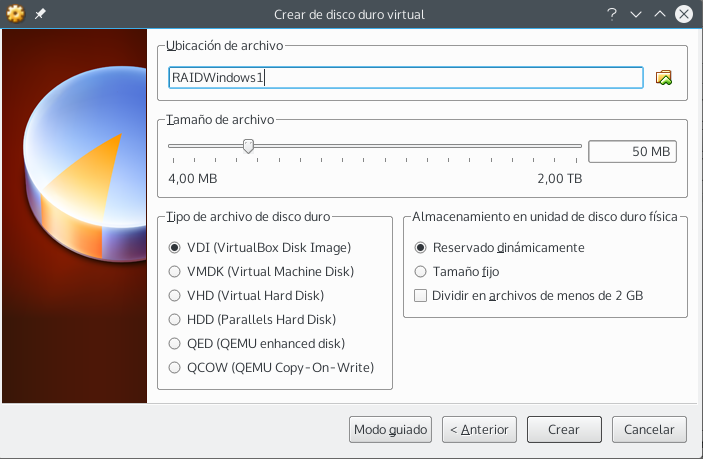
\includegraphics[width=0.5\textwidth]{11}
}
\qquad
\subfigure[Configuración final del almacenamiento del servidor Windows] {
\label{raidwin1}
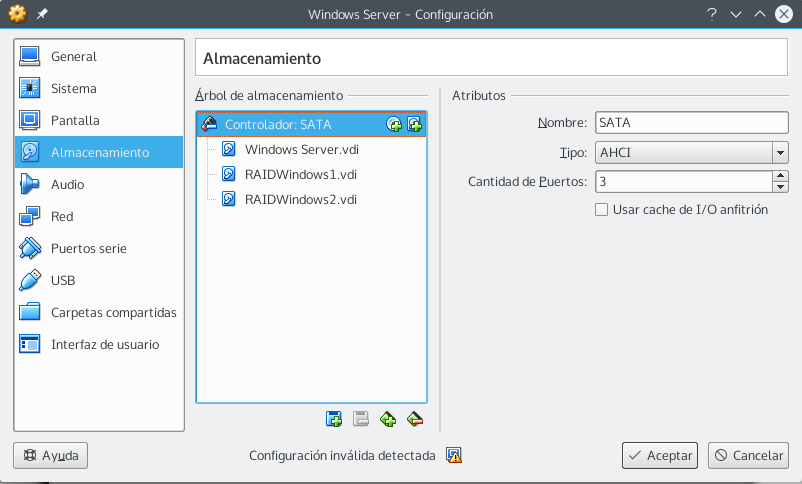
\includegraphics[width=0.5\textwidth]{12}
}
}
\caption{Añadiendo los discos virtuales para la creación del RAID1}
\label{raid1win}
\end{figure}

Tras esto, iniciamos la máquina virtual y abrimos la ventana \textbf{Administración de Equipos}, que se muestra en la \hyperref[admineq]{Figura \ref*{admineq}}, para ello seguimos la ruta \textbf{Inicio $>$ Herramientas de administración $>$ Administración de equipos}.

\begin{figure}[!h]
\centering
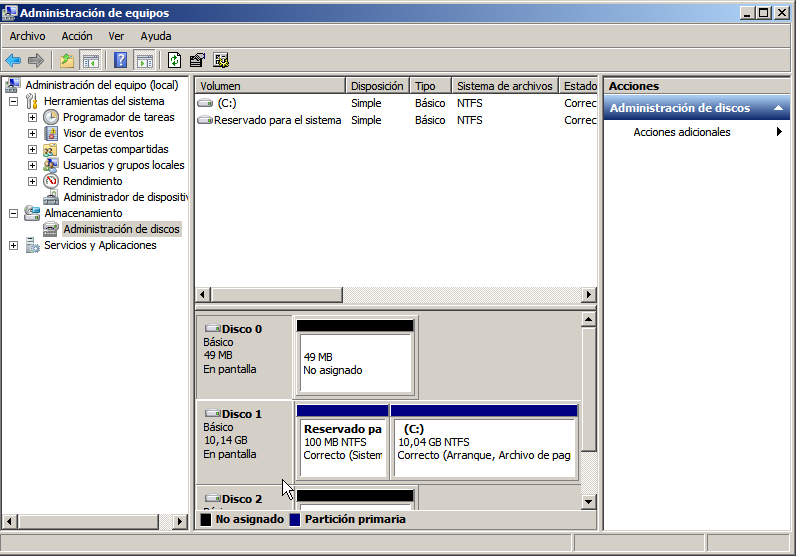
\includegraphics[width=0.5\textwidth]{13}
\caption{Ventana ``Administración de equipos''}
\label{admineq}
\end{figure}

Para crear el RAID1, seguimos la ruta mostrada en la \hyperref[ruta]{Figura \ref*{ruta}}: \textbf{Acción $>$ Todas las tareas $>$ Nuevo volumen reflejado...}

\begin{figure}[!h]
\centering
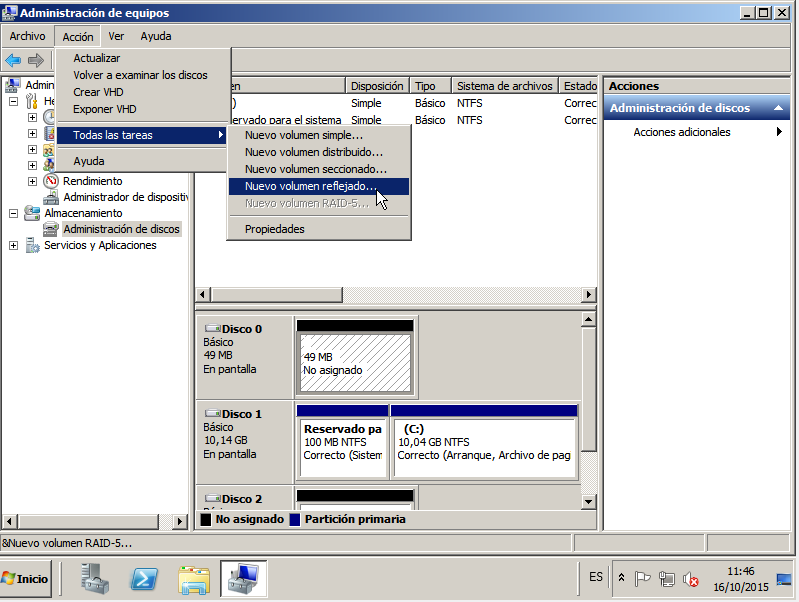
\includegraphics[width=0.5\textwidth]{14}
\caption{Ruta para crear un volumen reflejado}
\label{ruta}
\end{figure}

Tras esto, se nos abrirá un asistente que nos guiará en la creación del disco reflejado. Dicho asistente, nos pedirá en primer lugar que seleccionemos qué discos formarán parte del disco reflejado, tras seleccionarlo todo, debe quedar como se muestra en la \hyperref[discos]{Figura \ref*{discos}}.

\begin{figure}[!h]
\centering
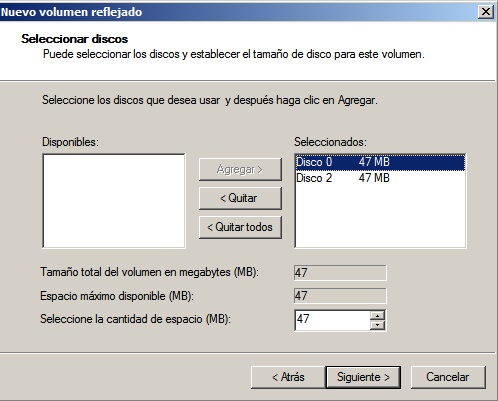
\includegraphics[width=0.5\textwidth]{15}
\caption{Selección de los discos que formarán el volumen reflejado}
\label{discos}
\end{figure}

Después asignaremos una letra a la unidad creada, en nuestro caso, lo dejaremos por defecto, como se ve en la \hyperref[letra]{Figura \ref*{letra}}.

\begin{figure}[!h]
\centering
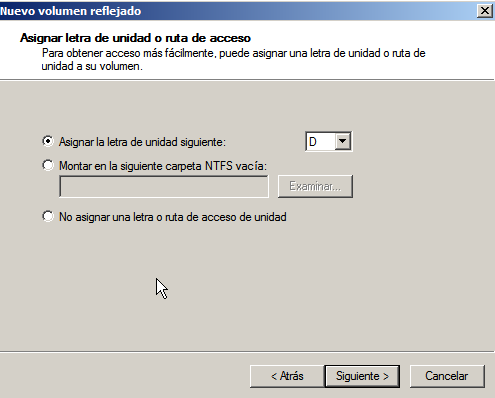
\includegraphics[width=0.5\textwidth]{16}
\caption{Asignación de una letra al volumen creado}
\label{letra}
\end{figure}

Tras asignar una letra, formatearemos el volumen creado con un sistema de archivos NTFS y un formateo rápido, como se ve en la \hyperref[formateo]{Figura \ref*{formateo}}.

\begin{figure}[!h]
\centering
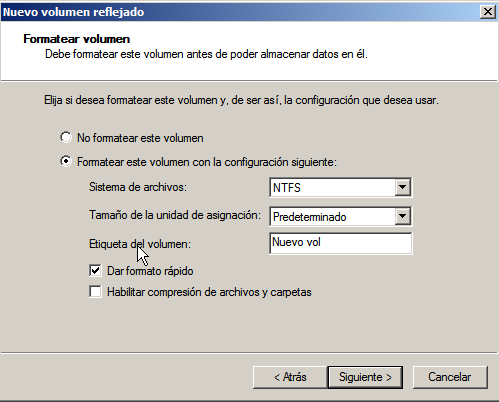
\includegraphics[width=0.5\textwidth]{17}
\caption{Formateo del volumen creado.}
\label{formateo}
\end{figure}

Después de formatear el volumen, finalizaremos el asistente y nos saldrá el mensaje de la \hyperref[mensaje]{Figura \ref*{mensaje}}, en el que seleccionaremos la opción \textbf{Sí}.

\begin{figure}[!h]
\centering
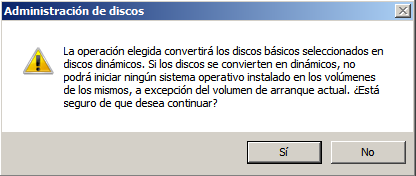
\includegraphics[width=0.5\textwidth]{19}
\caption{Mensaje tras finalizar la creación del volumen reflejado}
\label{mensaje}
\end{figure}

\section{Explique brevemente qué diferencias hay entre los tres tipos de conexión que permite el VMSW para las MVs: NAT, Host-only y Bridge}
En la documentación de VMWare, \cite{tiposconexion}, se explican los tres tipos de conexión disponibles:

\begin{description}
    \item[NAT]: siglas provenientes de \textit{Network Address Translation}, con este tipo de conexión la máquina virtual y el sistema host comparten la misma dirección IP, es decir, en la red actúan como un solo elemento. Así, podemos conectar la máquina virtual a internet sin tener una dirección IP exclusiva para la máquina virtual.

    \item[Host-only]: con host-only, creamos una conexión entre la máquina virtual y el sistema operativo host usando un adaptador de red virtual visible para el sistema operativo host. Así, la máquina virtual sólo podrá comunicarse con el sistema operativo host y otras máquinas virtuales que estén dentro de la red host-only. En resumidas cuentas, con la conexión host-only, creamos una red virtual aislada.

    \item[Bridge]: con la conexión Bridge, la máquina virtual tiene su propia dirección IP y actúa como un dispositivo más en la red. Por tanto, el resto de dispositivos de la red se pueden comunicar con la máquina virtual. 
\end{description}

Por tanto, viendo la definición de cada tipo de red, podemos decir que la principal diferencia está en el tipo de comunicación que existe entre el host y la máquina virtual:
\begin{enumerate}[---]
    \item Si el host se comunica con la máquina virtual de la misma forma que lo haría con otro equipo de la red, tenemos una conexión Bridge.
    \item Si en la red tienen la misma IP y por tanto el host tiene que diferenciar de los mensajes que son ``para él'' y los mensajes que no, tenemos una NAT
    \item Y si la máquina virtual no tiene comunicación con el ``mundo exterior'', sino que sólo se comunica con el host, tenemos una Host-only.
\end{enumerate}

\section{Cuestiones Opcionales}
\subsection{Muestre (con capturas de pantalla) cómo ha comprobado que el RAID1 funciona.}
Tras eliminar el disco 1 de la máquina virtual e iniciar el sistema, comprobamos que al arrancar obtenemos la pantalla de la \hyperref[raid1]{Figura \ref*{raid1}}

\begin{figure}[!h]
\centering
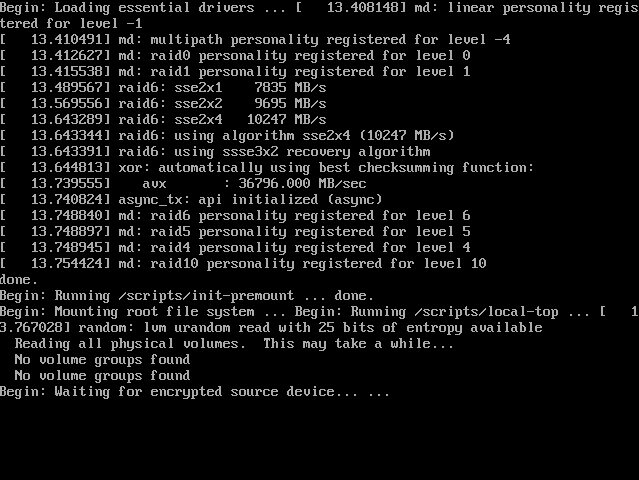
\includegraphics[width=0.8\textwidth]{7}
\caption{Pantalla al arrancar por primera vez habiendo quitado el disco 1}
\label{raid1}
\end{figure}

Tras esto, se iniciará el modo \texttt{initramfs}, en el que podremos ejecutar las instrucciones que se ven en la \hyperref[initramfs]{Figura \ref*{initramfs}} (obtenidas al pulsar el tabulador)

\begin{figure}[!h]
\centering
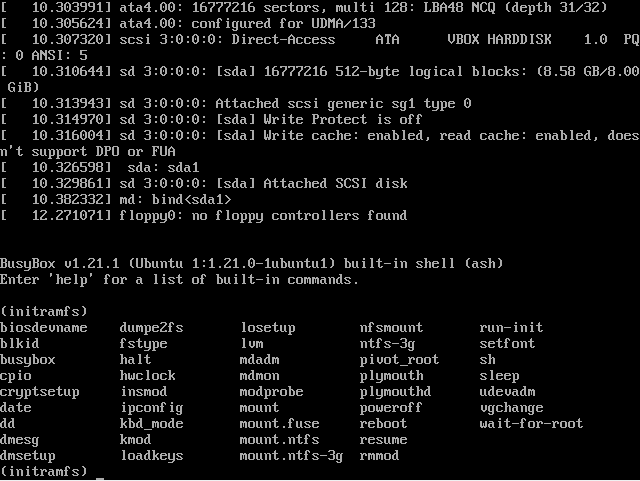
\includegraphics[width=0.8\textwidth]{8}
\caption{Pantalla al iniciarse \texttt{initramfs} y pulsar tabulador}
\label{initramfs}
\end{figure}

Comprobamos, en primer lugar, el estado actual en el que se encuentra el RAID consultado el archivo \texttt{mdstat}. Como se ve en la \hyperref[inactive]{Figura \ref*{inactive}}, vemos que está desactivado.

\begin{figure}[!h]
\centering
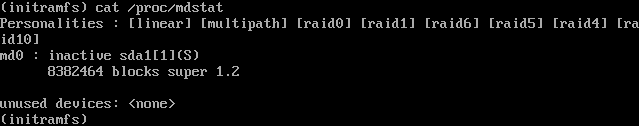
\includegraphics[width=0.8\textwidth]{10}
\caption{Comprobación del estado del RAID}
\label{inactive}
\end{figure}

Para activarlo, vamos a ejecutar \texttt{mdadm}, para ello ejecutamos tal y como se indica en las páginas man de \texttt{mdadm} (\cite{mdadm}):

\begin{minted}{bash}
mdadm -R /dev/md0
\end{minted}

Lo ejecutamos sobre md0, ya que estamos trabajando sobre el dispositivo RAID. Así, tal y como se ve en la \hyperref[active]{Figura \ref*{active}}, ya tenemos nuestro dispositivo RAID activado. 

Para terminar, pulsamos \textbf{Control+D} para seguir arrancando el sistema.

\begin{figure}[!h]
\centering
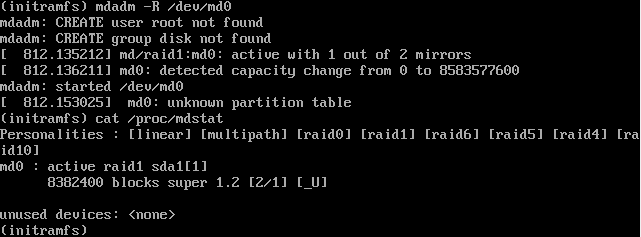
\includegraphics[width=0.8\textwidth]{9}
\caption{Activación del RAID y su posterior comprobación}
\label{active}
\end{figure}

\subsection{¿Qué relación hay entre los atajos de teclado de emacs y los de la consola de bash? ¿y entre los de vi y las páginas del manual?}
Tal y como se dice en \cite{keysemacs}, los atajos de teclado tanto en bash como en emacs son los mismos. También en \cite{keysemacs} nos ponen unos ejemplos de atajos de teclado de emacs para la consola de bash:
\begin{enumerate}[$\heartsuit$]
    \item \texttt{CTRL-P}: ir al comando anteriormente ejecutado en el historial
    \item \texttt{CTRL-N}: ir al siguiente comando ejecutado en el historial
    \item \texttt{CTRL-R}: buscar en el historial de comandos ejecutados al revés
    \item \texttt{CTRL-S}: según la página es buscar en el historial de comandos, pero a mí me suspende la terminal y tengo que pulsar \texttt{CTRL-Q} para volverla a iniciar.
    \item \texttt{CTRL-A}: mover el cursor al inicio de la línea.
    \item \texttt{CTRL-E}: mover el cursor al final de la línea
    \item \texttt{CTRL-W}: eliminar la última palabra en la que se encuentra el cursor. Por ejemplo, en el comando \texttt{bibtex citas}, eliminaría la palabra \texttt{citas}.
    \item \texttt{ALT-D}: eliminar la siguiente palabra a la que apunta el cursor. Por ejemplo, si tenemos el cursor al inicio de la línea, se eliminaría la primera palabra.
    \item \texttt{CTRL-F}: mover el cursor un carácter hacia delante.
    \item \texttt{CTRL-B}: mover el cursor un carácter hacia atrás.
    \item \texttt{ALT-F}: mover el cursor una palabra hacia delante.
    \item \texttt{ALT-B}: mover el cursor una palabra hacia detrás.
    \item \texttt{ALT-\_}: escribir la última palabra que has escrito en el historial.
\end{enumerate}

Lo mismo pasa con \texttt{vi} y las \texttt{man pages}. Por ejemplo, en la \hyperref[man]{Figura \ref*{man}} vemos los comandos para movernos por una página de manual, pero, esos mismos comandos también nos sirven para movernos por un archivo abierto con vi, pero combiándolos con la tecla control.

\begin{figure}[!h]
\centering
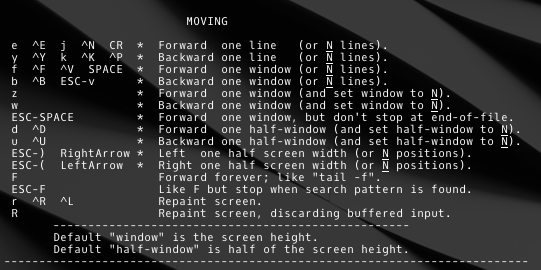
\includegraphics[width=0.5\textwidth]{20}
\caption{Comandos para moverse a través de una página de manual}
\label{man}
\end{figure}

\bibliography{P1-MarGomMac} %archivo citas.bib que contiene las entradas 
\bibliographystyle{siam} % hay varias formas de citar

\end{document}